\section{Simulation Results}%
\label{sec:simulations}

\begin{figure}[t]
    \centerline{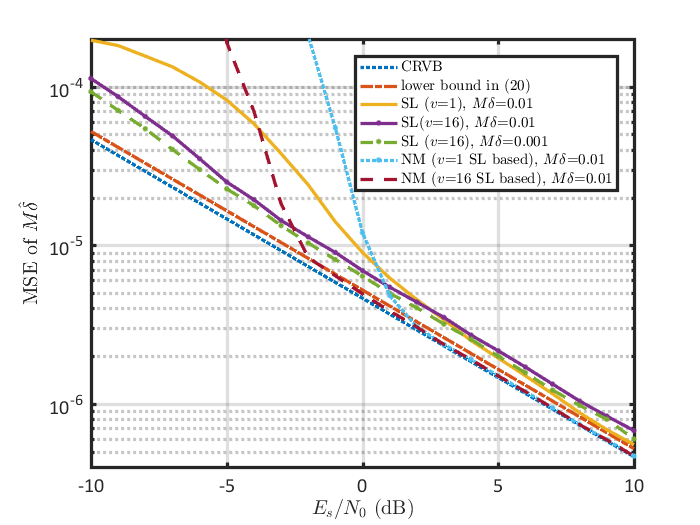
\includegraphics[width=3.15in]{accuracy_NM_SL.png}}
    \caption{Accuracy of the NM and the SL estimators ($L_0=32$, $M=2$)}
    \label{fig:accuracy_NM_SL}
    \end{figure}

In the simulation section, we reverse the order of discussion by first showing 
the accuracy of estimators in carrier synchronization and then showing some results of sequential detection since
the GLRT based detector in~\eqref{eq:generalized_corr} relies on the accuracy of 
the SL estimator.
The symbol sequence of the preamble is chosen as a Gold sequence 
with good autocorrelation properties and
modulated by a QPSK alphabet.
The pulse is chosen a
Square-Root Raised Cosine (SRRC) pulse with roll-off equal to 0.5.
The normalized frequency offset $\delta$ is intentionally set to be in
the safe estimation range for all estimators for simulation purposes. 

\subsection{Simulation Results for Estimation}%

% \begin{figure}[t]
%     \centerline{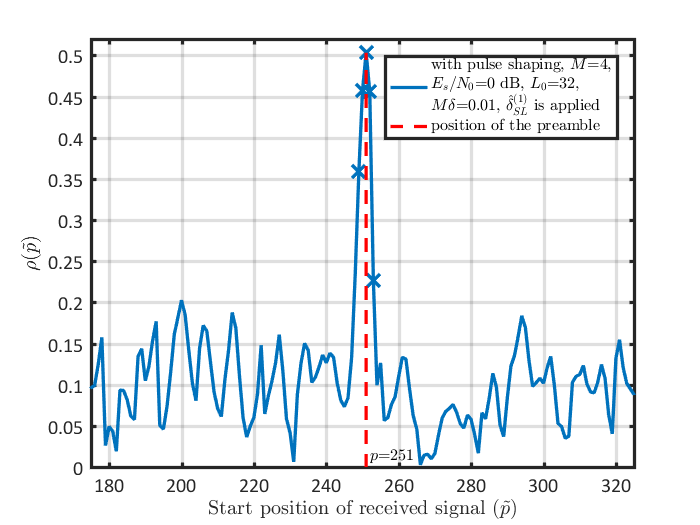
\includegraphics[width=3.4in]{generalized_correlation_p_plus_delta.png}}
%     \caption{Performance of sequential detector when the preamble is pulse shaped}
%     \label{fig:Generalized correlation}
%     \end{figure}

Figure~\ref{fig:accuracy_NM_SL} illustrates the accuracy of the single-lag (SL) and the NM estimator.
Comparing the two curves for SL estimators with $v=1$ and $v=32$, 
we see the length-$32$ partial integration
improves the accuracy by providing an approximate
\SI{4}{\dB}~performance gain at negative SNRs
(near $\text{SNR}=\SI{-5}{\dB}$). This is consistent
with~\eqref{eq:relative_processing_gain}.

The SL estimator with $v=1$ is slightly more accurate
at \SI{10}{\dB}~SNR than with $v=32$.
The gap is due to the Dirichlet function.
% for $\delta \neq 0$.
For the same reason,
when $v>1$
the accuracy of the estimator improves at all SNRs as $|\delta|$ decreases.
% When  $\delta$ is very small, the accuracy of the SL estimator with $v=32$ has better accuracy at all SNRs.

The SL estimators do not approach the Cramer-Rao Vector Bound (CRVB)~\cite{Gini_98} while the NM
estimators do at moderate SNR. 
% We also see that the
The NM estimator achieves improved accuracy at lower SNR
when the SL estimator with $v=32$ is used as the starting point. 
In contrast, at all negative SNRs the NM estimator based on SL estimation with $v=1$ has
worse accuracy than SL estimation alone.
This is because the accuracy of the SL estimator is not sufficient to
provide a consistently good starting point and the Newton iteration converges occasionally to 
other local minima away from the true frequency offset.

Figure~\ref{fig:accuracy_NM_SL_traditional} compares the accuracy of our proposed estimators
and the estimators in~\cite{kay_89,Fitz_94,Luise_Reggiannini_95}.
When the 
frequency offset is small, our NM estimator has a slightly better accuracy than other estimators at moderate SNRs.
In general, our family of  SL estimators with different block lengths $v$
are very competitive across all SNRs considered here while maintaining
low computational complexity that allows for real-time application.

\begin{figure}[t]
    \centerline{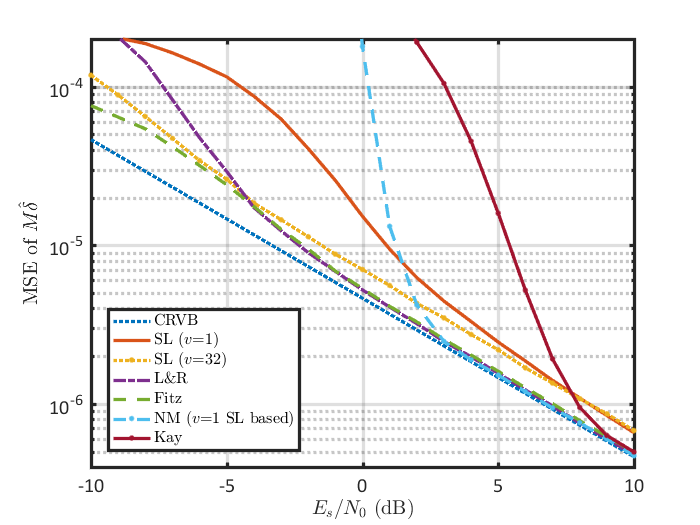
\includegraphics[width=3.15in]{accuracy_NM_SL_traditional.png}}
    \caption{Accuracy of the SL, the NM and the traditional estimators ($L_0=32$, $M=2$, $M\delta=0.01$)}
    \label{fig:accuracy_NM_SL_traditional}
    \end{figure}

\begin{figure}[t]
  \centerline{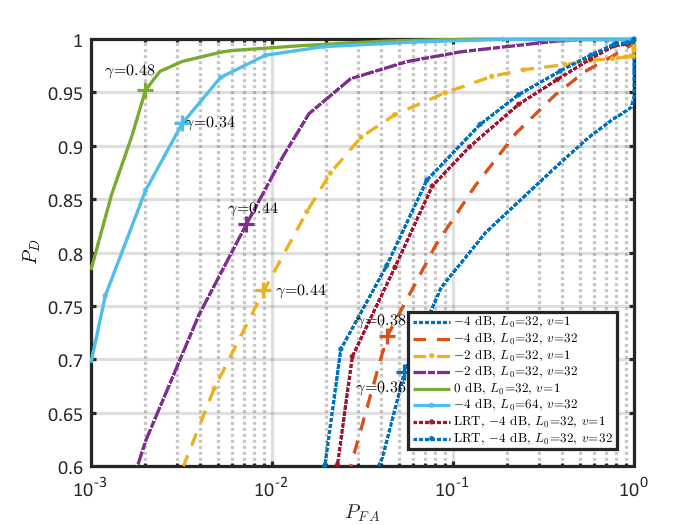
\includegraphics[width=3.15in]{ROC_new.png}}
  \caption{Receiver operating characteristics (ROC) of the sequential detector ($M=2$, $M\delta=0.01$)}
  \label{fig:Receiver operating characteristics}
\end{figure}


\subsection{Simulation Results for Detection}

% Figure~\ref{fig:Generalized correlation} shows the performance of sequential detector
% in~\eqref{eq:generalized_corr} at each received signal windows. Note, because of pulse sha-ping,
% the autocorrelation property of the preamble sequence is decreased, which results
% the correlations at adjacent windows near the position of the preamble decay slow and thus make much challenges
% to choose threshold to make correct dicision.

% The solution is to adjust the detection algorithm by finding the local maximum of the correlation
% instead of just comparing the correlation with the threshold at each window. Note, when count for the ratio of false alarm and detection (for determining the threshold),
% the two positions should be counted as latter.


Figure~\ref{fig:Receiver operating characteristics} shows the receiver
operating characteristics (ROC) of the detection algorithm. 
The better accuracy of SL estimation with partial integration also
improves the detection performance  at low SNR.
For example, at $\SI{-2}{\dB}$ SNR, $\gamma=0.44$, the false alarm probability $P_{FA}$ of SL with $v=32$ is reduced $0.2\%$ and 
the detection probability $P_{D}$ is $5\%$ larger compared with the SL with $v{=}1$. 
The figure also shows the detector does not work well at $\SI{-4}{\dB}$ SNR if only $32$ symbols of preamble are used;  
The performance is significantly improved by doubling the length of
the preamble. The two curves marked LRT at $\SI{-4}{\dB}$ SNR with different $v$
are obtained by plugging in the true frequency and phase offsets as an upper bound for comparing with 
the results of the GLRT.   

% \begin{figure}[t]
%   \centerline{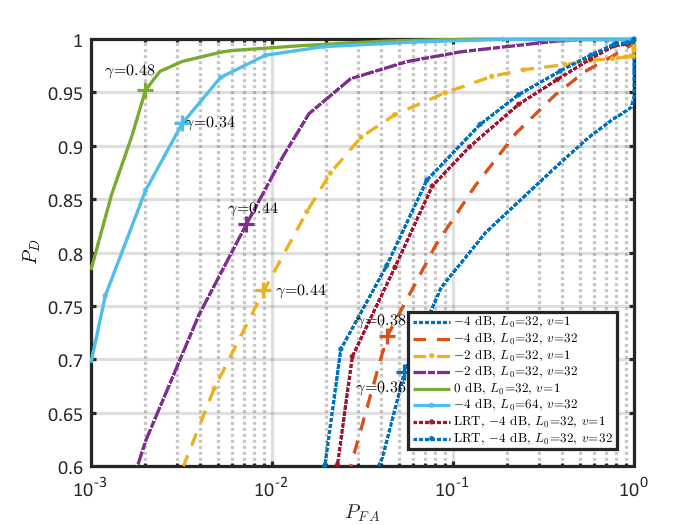
\includegraphics[width=3.15in]{ROC_new.png}}
%   \caption{Receiver operating characteristics (ROC) of the sequential detector ($M=2$, $M\delta=0.01$)}
%   \label{fig:Receiver operating characteristics}
% \end{figure}

